\documentclass[10pt]{article}

\usepackage[letterpaper,margin=0.62in]{geometry}
\usepackage[T1]{fontenc}
\usepackage[utf8]{inputenc}
\usepackage{mathpazo}
\usepackage[scaled=0.94]{helvet}
\usepackage{courier}
\usepackage{microtype}
\usepackage{graphicx}
\usepackage{hyperref}
\usepackage[most]{tcolorbox}
\usepackage{tikz}
\usetikzlibrary{arrows.meta,calc,positioning}
\usepackage{tabularx}
\usepackage{ragged2e}
\usepackage{xcolor}
\usepackage{enumitem}

\definecolor{Ink}{HTML}{09171D}
\definecolor{InkSoft}{HTML}{13282F}
\definecolor{Slate}{HTML}{40525A}
\definecolor{Muted}{HTML}{73858B}
\definecolor{Jade}{HTML}{08A88A}
\definecolor{JadeDark}{HTML}{087563}
\definecolor{Cyan}{HTML}{43D6CC}
\definecolor{Paper}{HTML}{F6F4EE}
\definecolor{PaperCool}{HTML}{EEF5F2}
\definecolor{White}{HTML}{FFFFFF}
\definecolor{Line}{HTML}{CCD9D5}
\definecolor{Warn}{HTML}{D6A84A}

\hypersetup{
  colorlinks=true,
  linkcolor=JadeDark,
  urlcolor=JadeDark
}

\pagestyle{empty}
\setlength{\parindent}{0pt}
\setlength{\parskip}{0.45em}
\setlist[itemize]{leftmargin=1.25em,itemsep=0.2em,topsep=0.25em}
\RaggedRight

\newcommand{\eyebrow}[1]{%
  {\sffamily\bfseries\footnotesize\color{Jade}\MakeUppercase{#1}}%
}

\newcommand{\pagetitle}[1]{%
  {\sffamily\bfseries\fontsize{27}{29}\selectfont\color{Ink}#1\par}%
}

\newcommand{\pagesubtitle}[1]{%
  {\sffamily\fontsize{11.5}{15}\selectfont\color{Slate}#1\par}%
}

\newcommand{\pageheader}[2]{%
  \noindent
  \begin{tabularx}{\textwidth}{@{}p{0.7in}Xr@{}}
    {\sffamily\bfseries\color{Jade}#1} &
    {\sffamily\bfseries\color{Ink}#2} &
    {\sffamily\footnotesize\color{Muted}KUNGFU WHITE PAPER \textperiodcentered{} VISUAL PROOF}
  \end{tabularx}
  \vspace{0.14in}
  {\color{Line}\hrule height 0.6pt}
  \vspace{0.28in}
}

\newcommand{\pagefooter}[1]{%
  \begin{tikzpicture}[remember picture,overlay]
    \draw[Line,line width=0.6pt]
      ([xshift=0.62in,yshift=0.48in]current page.south west) --
      ([xshift=-0.62in,yshift=0.48in]current page.south east);
    \node[anchor=west,font=\sffamily\footnotesize,text=Muted]
      at ([xshift=0.62in,yshift=0.29in]current page.south west)
      {Kungfu Origin Technology Limited};
    \node[anchor=east,font=\sffamily\bfseries\footnotesize,text=JadeDark]
      at ([xshift=-0.62in,yshift=0.29in]current page.south east) {#1};
  \end{tikzpicture}%
}

\newtcolorbox{softcard}[1][]{
  enhanced,
  colback=White,
  colframe=Line,
  boxrule=0.6pt,
  arc=2.2mm,
  left=3.5mm,right=3.5mm,top=3mm,bottom=3mm,
  #1
}

\newtcolorbox{darkcard}[1][]{
  enhanced,
  colback=InkSoft,
  colframe=InkSoft,
  boxrule=0pt,
  arc=2.2mm,
  left=4mm,right=4mm,top=3.5mm,bottom=3.5mm,
  #1
}

\newcommand{\separationcard}[3]{%
  \begin{minipage}[t]{0.485\textwidth}
  \begin{softcard}
    {\sffamily\bfseries\footnotesize\color{Jade}#1}\par
    {\sffamily\bfseries\fontsize{11.5}{13}\selectfont\color{Ink}#2}\par
    {\small\color{Slate}#3}
  \end{softcard}
  \end{minipage}%
}

\newcommand{\kfdrow}[4]{%
  \begin{softcard}[colback=#4]
  \begin{tabularx}{\linewidth}{@{}p{0.72in}X@{}}
    {\sffamily\bfseries\fontsize{17}{18}\selectfont\color{JadeDark}#1} &
    {\sffamily\bfseries\fontsize{15}{17}\selectfont\color{Ink}#2}\par
    {\small\color{Slate}#3}
  \end{tabularx}
  \end{softcard}
}

\newcommand{\architecturelayer}[3]{%
  \begin{softcard}[colback=#3,left=3mm,right=3mm,top=2.5mm,bottom=2.5mm]
    {\sffamily\bfseries\fontsize{12}{13}\selectfont\color{Ink}#1}\par
    {\small\color{Slate}#2}
  \end{softcard}
}

\newcommand{\ladderrow}[3]{%
  \noindent
  \begin{tabularx}{\linewidth}{@{}p{0.32in}X@{}}
    \tikz[baseline=(n.base)]\node[fill=#3,text=White,circle,inner sep=2.3pt,
      font=\sffamily\bfseries\scriptsize] (n) {#1}; &
    {\sffamily\bfseries\small\color{Ink}#2}
  \end{tabularx}
  \vspace{0.11in}
}

\begin{document}

% ---------------------------------------------------------------------------
% Page 1: cover
% ---------------------------------------------------------------------------
\pagecolor{Ink}
\begin{tikzpicture}[remember picture,overlay]
  \fill[Jade] (current page.north east) rectangle
    ([xshift=-0.17in]current page.south east);
  \draw[Cyan,opacity=0.22,line width=1.2pt]
    ([xshift=-0.9in,yshift=-1.0in]current page.north east)
    .. controls ([xshift=-2.7in,yshift=-2.2in]current page.north east)
    and ([xshift=-1.2in,yshift=2.0in]current page.south east)
    .. ([xshift=-3.4in,yshift=0.8in]current page.south east);
  \draw[Jade,opacity=0.13,line width=30pt]
    ([xshift=-0.45in,yshift=-0.9in]current page.north east) --
    ([xshift=-3.0in,yshift=0.7in]current page.south east);
  \foreach \y in {1.5,2.4,3.3,4.2} {
    \fill[Cyan,opacity=0.15]
      ([xshift=-0.82in,yshift=\y in]current page.south east) circle (0.055in);
  }
\end{tikzpicture}

{\sffamily\bfseries\footnotesize\color{Cyan}KUNGFU WHITE PAPER \textperiodcentered{} JULY 2026}\par
\vspace{1.15in}

{\sffamily\bfseries\fontsize{43}{45}\selectfont\color{White}
Kungfu:\par
Continuity for\par
Agent Work\par}

\vspace{0.35in}
{\color{Jade}\rule{1.05in}{3pt}}\par
\vspace{0.28in}

{\sffamily\fontsize{16}{21}\selectfont\color{PaperCool}
A local-first product and runtime for Projects, Work,\par
and replaceable Agents.\par}

\vfill


\begin{tikzpicture}[node distance=0.18in]
  \tikzset{
    covernode/.style={rounded corners=2pt,draw=Cyan!35,fill=InkSoft,
      text=White,minimum width=1.34in,minimum height=0.48in,
      align=center,font=\sffamily\bfseries\small},
    coverarrow/.style={-{Stealth[length=5pt]},draw=Jade,line width=1.1pt}
  }
  \node[covernode] (a) {Chat ends};
  \node[covernode,right=of a] (b) {Work remains};
  \node[covernode,right=of b] (c) {Fresh Agent};
  \node[covernode,right=of c] (d) {Independent review};
  \draw[coverarrow] (a) -- (b);
  \draw[coverarrow] (b) -- (c);
  \draw[coverarrow] (c) -- (d);
\end{tikzpicture}

\vspace{0.55in}
{\sffamily\bfseries\fontsize{14}{18}\selectfont\color{White}
Work should not disappear when a chat ends, restart when an Agent changes,\par
or become complete merely because a process exits.\par}

\vspace{0.55in}
\begin{tabularx}{\textwidth}{@{}Xr@{}}
  {\sffamily\color{PaperCool}Keren Dong\par
   \footnotesize Kungfu Origin Technology Limited} &
  {\sffamily\footnotesize\color{Cyan}kungfu.tech \textperiodcentered{} kfd.libkungfu.dev}
\end{tabularx}

\newpage
\pagecolor{Paper}

% ---------------------------------------------------------------------------
% Page 2: product proof
% ---------------------------------------------------------------------------
\pageheader{01}{THE FIRST PROOF}
\eyebrow{Product promise}\par
\vspace{0.08in}
\pagetitle{The chat ended. The Work did not.}
\vspace{0.12in}
\pagesubtitle{Two genuinely fresh processes continue one governed Work without
transcript transfer. The result is visible before the ontology is explained.}

\vspace{0.23in}
\begin{tcolorbox}[
  enhanced,colback=Ink,colframe=Ink,boxrule=0pt,arc=2.5mm,
  left=2.5mm,right=2.5mm,top=2.5mm,bottom=2.5mm]
  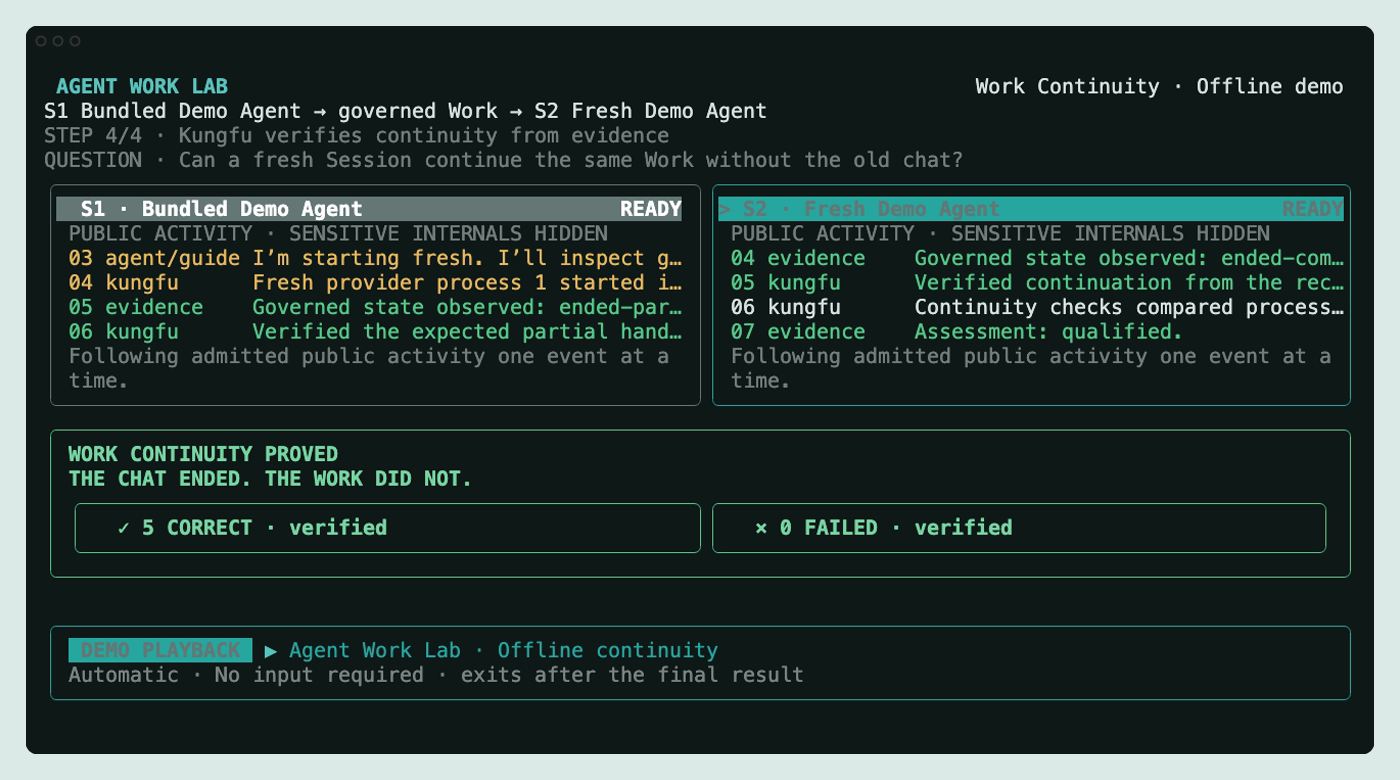
\includegraphics[width=\linewidth]{assets/agent-work-lab-continuity.png}
\end{tcolorbox}

\vspace{0.08in}
{\sffamily\footnotesize\color{Muted}
Installed Kungfu Agent Work Lab \textperiodcentered{} 5 continuity checks verified
\textperiodcentered{} 0 failures.
This is bounded artifact evidence, not yet longitudinal production proof.}

\vspace{0.24in}
\separationcard{01}{Work identity $\neq$ Agent process identity}
{A fresh process can enter the same bounded outcome rather than reconstructing
it from conversation.}
\hfill
\separationcard{02}{Admitted fact $\neq$ model output}
{Observations and claims remain evidence until assessment and admission justify
their use.}

\vspace{0.12in}
\separationcard{03}{Capability $\neq$ authority}
{An Agent may be able to publish while remaining unauthorized to publish this
candidate at this cut.}
\hfill
\separationcard{04}{Process success $\neq$ completion}
{Exit status and green CI can contribute evidence without closing the Work they
are supposed to prove.}

\pagefooter{02}

\newpage

% ---------------------------------------------------------------------------
% Page 3: foundation and agent reading instrument
% ---------------------------------------------------------------------------
\pageheader{02}{THE FOUNDATION TRIAD}
\eyebrow{Foundation before ontology}\par
\vspace{0.08in}
\pagetitle{Three obligations\\hold the world together.}
\vspace{0.1in}
\pagesubtitle{The Triad is not a feature list. It establishes the conditions
for a shared world, a trustworthy judgment, and useful cooperation.}

\vspace{0.2in}
\kfdrow{KFD-1}{Facts must not drift.}
{Declare the fact source and expose the cut when source, runtime, Work identity,
or evidence diverges.}{White}
\vspace{0.08in}
\kfdrow{KFD-2}{Trust must start from facts.}
{Evidence, claim, assessment, authority, and completion remain distinct so that
reliance and residual risk stay inspectable.}{PaperCool}
\vspace{0.08in}
\kfdrow{KFD-3}{Cooperation must start from trusted value.}
{Useful outcomes, choices, constraints, authority, and review paths are visible
before participants cooperate.}{White}

\vspace{0.2in}
\begin{tcolorbox}[
  enhanced,colback=Ink,colframe=Ink,boxrule=0pt,arc=2.5mm,
  left=4.2mm,right=4.2mm,top=3.5mm,bottom=3.5mm]
  {\sffamily\bfseries\fontsize{13}{15}\selectfont\color{Cyan}
  Explore KFD with an Agent}\par
  {\small\color{PaperCool}
  You do not need to memorize the internal ontology. Read the authoritative
  \href{https://kfd.libkungfu.dev/foundation/}{KFD Foundation Model}, or give
  this bounded prompt to an Agent:}\par
  \vspace{0.08in}
  {\ttfamily\fontsize{8.1}{10.2}\selectfont\color{White}
  Using the ``Publish a Public Alpha'' example, explain Project / Work / Agent,
  then Fact / Episode, then Pursuit / Atlas / Warrant, then Assessment /
  Decision / Admission / Project Cut. For each layer: what fails without it,
  which distinction it preserves, where it appears in the example, and what
  authority it does not possess. Separate KFD definitions from interpretation;
  pause after each layer.}
\end{tcolorbox}

\pagefooter{03}

\newpage

% ---------------------------------------------------------------------------
% Page 4: architecture and evidence
% ---------------------------------------------------------------------------
\pageheader{03}{HOW CONTINUITY WORKS}
\eyebrow{One core \textperiodcentered{} multiple complete products}\par
\vspace{0.08in}
\pagetitle{Higher layers expose value.\\Lower layers retain authority.}
\vspace{0.18in}

\begin{minipage}[t]{0.57\textwidth}
  {\sffamily\bfseries\fontsize{14}{16}\selectfont\color{Ink}Four product layers}\par
  {\small\color{Muted}The ordinary path stays small while deeper mechanisms
  appear only when explanation or review requires them.}\par
  \vspace{0.12in}

  \architecturelayer{Product experience}
  {Project, Work, and Agent form the complete first layer.}{White}
  \begin{center}\color{Jade}$\downarrow$\end{center}
  \architecturelayer{Semantic and action runtime}
  {Fact and Episode retain state and causal experience. Pursuit, Atlas, and
  Warrant bind direction, perspective, and authority.}{PaperCool}
  \begin{center}\color{Jade}$\downarrow$\end{center}
  \architecturelayer{Responsibility and settlement}
  {Initiative, Assignment, assessment, decision, admission, and Project Cut
  govern ownership and completion.}{White}
  \begin{center}\color{Jade}$\downarrow$\end{center}
  \architecturelayer{Supply chain and extension}
  {KFD, Buildchain, libkungfu, KFX, and Agent Hubs preserve independent
  authorities across construction and transport.}{PaperCool}

  \vspace{0.15in}
  \begin{softcard}[colback=Ink,colframe=Ink]
    {\sffamily\bfseries\color{Cyan}The action loop}\par
    {\small\color{White}
    Fact cut $\rightarrow$ Pursuit $\rightarrow$ Atlas $\rightarrow$ Warrant
    $\rightarrow$ act $\rightarrow$ Episode $\rightarrow$ assess and admit
    $\rightarrow$ next Fact cut.}
  \end{softcard}
\end{minipage}
\hfill
\begin{minipage}[t]{0.38\textwidth}
  {\sffamily\bfseries\fontsize{14}{16}\selectfont\color{Ink}Evidence ladder}\par
  {\small\color{Muted}Every claim stops at the highest evidence class it has
  actually earned.}\par
  \vspace{0.18in}

  \ladderrow{1}{Contract evidence}{JadeDark}
  \ladderrow{2}{Source qualification}{JadeDark!88}
  \ladderrow{3}{Installed-artifact evidence}{JadeDark!76}
  \ladderrow{4}{Provider-bound evidence}{JadeDark!64}
  \ladderrow{5}{Longitudinal evidence}{JadeDark!52}
  \ladderrow{6}{Independent adoption evidence}{JadeDark!40}

  \vspace{0.14in}
  \begin{softcard}[colback=White]
    {\sffamily\bfseries\color{Ink}Current boundary}\par
    {\small\color{Slate}
    Kungfu has source-built product surfaces and exact installed-artifact
    evidence for the bounded Agent Work Lab path. It does not yet establish
    general production continuity, every platform, or independent adoption.}
  \end{softcard}
\end{minipage}

\pagefooter{04}

\newpage
\pagecolor{Ink}

% ---------------------------------------------------------------------------
% Page 5: conclusion and research bridge
% ---------------------------------------------------------------------------
\begin{tikzpicture}[remember picture,overlay]
  \draw[Jade,opacity=0.15,line width=55pt]
    ([xshift=-1.2in,yshift=0.4in]current page.north east) --
    ([xshift=-0.4in,yshift=-1.8in]current page.south west);
  \draw[Cyan,opacity=0.22,line width=1.2pt]
    ([xshift=0.5in,yshift=1.7in]current page.south west)
    .. controls ([xshift=3.2in,yshift=2.8in]current page.south west)
    and ([xshift=-2.7in,yshift=-2.4in]current page.north east)
    .. ([xshift=-0.5in,yshift=-1.1in]current page.north east);
\end{tikzpicture}

\begin{tabularx}{\textwidth}{@{}Xr@{}}
  {\sffamily\bfseries\footnotesize\color{Cyan}04 \textperiodcentered{} THE RESEARCH BRIDGE} &
  {\sffamily\footnotesize\color{PaperCool}KUNGFU WHITE PAPER \textperiodcentered{} VISUAL PROOF}
\end{tabularx}
\vspace{0.14in}
{\color{Jade}\hrule height 0.8pt}

\vspace{0.75in}
{\sffamily\bfseries\fontsize{36}{39}\selectfont\color{White}
Work can survive\par
the Agent.\par}

\vspace{0.25in}
{\sffamily\fontsize{14}{19}\selectfont\color{PaperCool}
Kungfu preserves Work identity, evidence, responsibility, and continuation
across replaceable Agent processes. That is the present product claim.\par}

\vspace{0.52in}
\begin{minipage}[t]{0.46\textwidth}
  \begin{darkcard}
    {\sffamily\bfseries\footnotesize\color{Cyan}PRESENT PRODUCT}\par
    {\sffamily\bfseries\fontsize{17}{19}\selectfont\color{White}
    Continuity for Agent Work}\par
    \vspace{0.1in}
    {\small\color{PaperCool}
    Project / Work / Agent\par
    Fact and Episode\par
    Bounded authority\par
    Independent completion\par
    Inspectable evidence}
  \end{darkcard}
\end{minipage}
\hfill
\begin{minipage}[t]{0.46\textwidth}
  \begin{darkcard}
    {\sffamily\bfseries\footnotesize\color{Warn}FUTURE RESEARCH}\par
    {\sffamily\bfseries\fontsize{17}{19}\selectfont\color{White}
    Continuity for a machine subject?}\par
    \vspace{0.1in}
    {\small\color{PaperCool}
    Replaceable cognition\par
    Candidate organs\par
    Selection membranes\par
    Successor cuts\par
    Governed self-production}
  \end{darkcard}
\end{minipage}

\vspace{0.48in}
\begin{center}
  {\sffamily\bfseries\fontsize{19}{23}\selectfont\color{Cyan}
  Can the same organization let a subject survive replacement\par
  of the machinery through which it thinks and acts?}
\end{center}

\vfill
{\color{Jade}\hrule height 0.8pt}
\vspace{0.14in}
\begin{tabularx}{\textwidth}{@{}Xr@{}}
  {\sffamily\footnotesize\color{PaperCool}
  Work continuity is a prerequisite for a persistent machine subject,\par
  not proof that one exists.} &
  {\sffamily\bfseries\footnotesize\color{Cyan}
  kungfu.tech \textperiodcentered{} kfd.libkungfu.dev}
\end{tabularx}

\end{document}
